\documentclass[11pt,a4paper]{article}
\usepackage[utf8]{inputenc}
\usepackage[english]{babel}

\usepackage{graphicx}
\usepackage[english]{babel}
\usepackage[margin=0.85in]{geometry}
\usepackage{amsmath}
\usepackage{amssymb}
\usepackage{natbib}
\usepackage{hyperref}
\bibliographystyle{plainnat}
\usepackage{setspace}


% These are the configurable settings
% Please change them to make it fit your course
\def \institute {Institute / project name}
\def \authors { Youri Hoogstrate, \institute }

\def \servers {
\begin{itemize}
	\item \url{https://usegalaxy.org/}
	\item \url{https://bioinf-galaxian.erasmusmc.nl/galaxy/}
\end{itemize}
}
\def \datalibrarydirintroduction {
	TraIT Galaxy Training Materials
		$\rightarrow$
	TraIT Galaxy Training - 1: Introduction to Galaxy
}

\def \datalibrarydirrnaseqtuxedo {
	TraIT Galaxy Training Materials
		$\rightarrow$
	TraIT Galaxy Training - 3: RNASeq Tuxedo Pipeline
}

\def \datalibrarydirrnaseqadvanced {
	TraIT Galaxy Training Materials
		$\rightarrow$
	TraIT Galaxy Training - 5: Advanced RNA-Seq Analysis
}
% Configurations should be changed in this file

\begin{document}
\title{ \textit{\institute}\text{ }Galaxy Training: RNA-Seq DGE analysis \\
{ \large This practical aims to familiarize you with the Galaxy RNA-Seq analysis, the FastQ format and data collections (pairs).}}

\author{ \authors }
\maketitle

%\newpage
%\tableofcontents
%\newpage

%\doublespacing

\section*{Introduction}
Due to the rapid development of Galaxy, screenshots and results may be out of date. If you experience something like this, please report it as a bug at \url{https://github.com/ErasmusMC-Bioinformatics/galaxy-courses/issues}.


% It should describe:
% - server address(es)
% - whether to use specific training accounts or register one
% - a notice until when the server will be available or whether it will be accessible after the course
% - funding related notices
\section*{Preparations}
\subsection*{Open Galaxy}
Please open a web browser and navigate to your assigned Galaxy server:

\servers

\subsection*{Register for an account}
In the top menu bar, go to User and then choose Register (fig. \ref{fig:registration}). After registration, click on Analyze data in the top menu to return to the main screen.

\begin{figure}
 \center
  
\includegraphics[scale=0.6]{../figures/register_icon_1}
  \caption{\small{ The icons used in Galaxy to go to the registration page }}
  \label{fig:registration}
\end{figure}% Preparations should describe how to access which server

% Module QC/QA:
\section{RNA-Seq: QC/QA}
The very first step of an RNA-Seq analysis is the quality control and quality assurance. The sequencing data is usually provided in FASTQ format, which reports the sequenced bases and also describes per base the quality reflecting the probability it was measured correctly. However, different encodings are being used. Galaxy contains tools that assist you in determining and dealing with these formats by converting them to \textit{fastqsanger}.

\subsection{Paired end data as `pairs' within galaxy}
\textbf{Note: using `pairs' for storing paired end reads in galaxy is experimental but will become the common way doing analysis on paired end data.} \\
This section will only show how to do this.

For this module, create a new history and load the Shared Data (\textit{\datalibrarydirrnaseqadvanced}) files ``ctrl\_small\_1.fq'' and ``ctrl\_small\_2.fq'' and ``treat\_small\_1.fq'' and ``treat\_small\_2.fq'' into your history. As you may expect from the file names already, \verb|_1| and \verb|_2| indicate that these files are paired end and belong together:\\
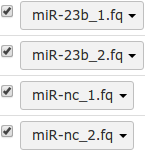
\includegraphics[scale=0.65]{figures/qc_01.png}\\
Hence, each pair of files belong to each other and we can treat them as pairs in galaxy. First you have to select the checkbox on top of the history ``\textit{Operations on multiple datasets}'', select the history items that belong to the pair of interest and then press the button \textit{For all selected...} to apply actions on multiple history items at once, select \textit{Build Dataset Pair}. Galaxy does not really know which one is the forward and which one is the reverse. Therefore make sure that \textbf{\_1 is forward} and \textbf{\_2 is reverse}. If galaxy does not choose the files correctly by it itself, use \text{Swap}. One of the samples has been treated with miR-23b and the other is a control. Make sure you use names that make this clear. After you have done this, you will see that you end up with 6 datasets in total, of which 2 pairs. To avoid confusion it is easier to hide the individual history items, leaving two items in the history:\\
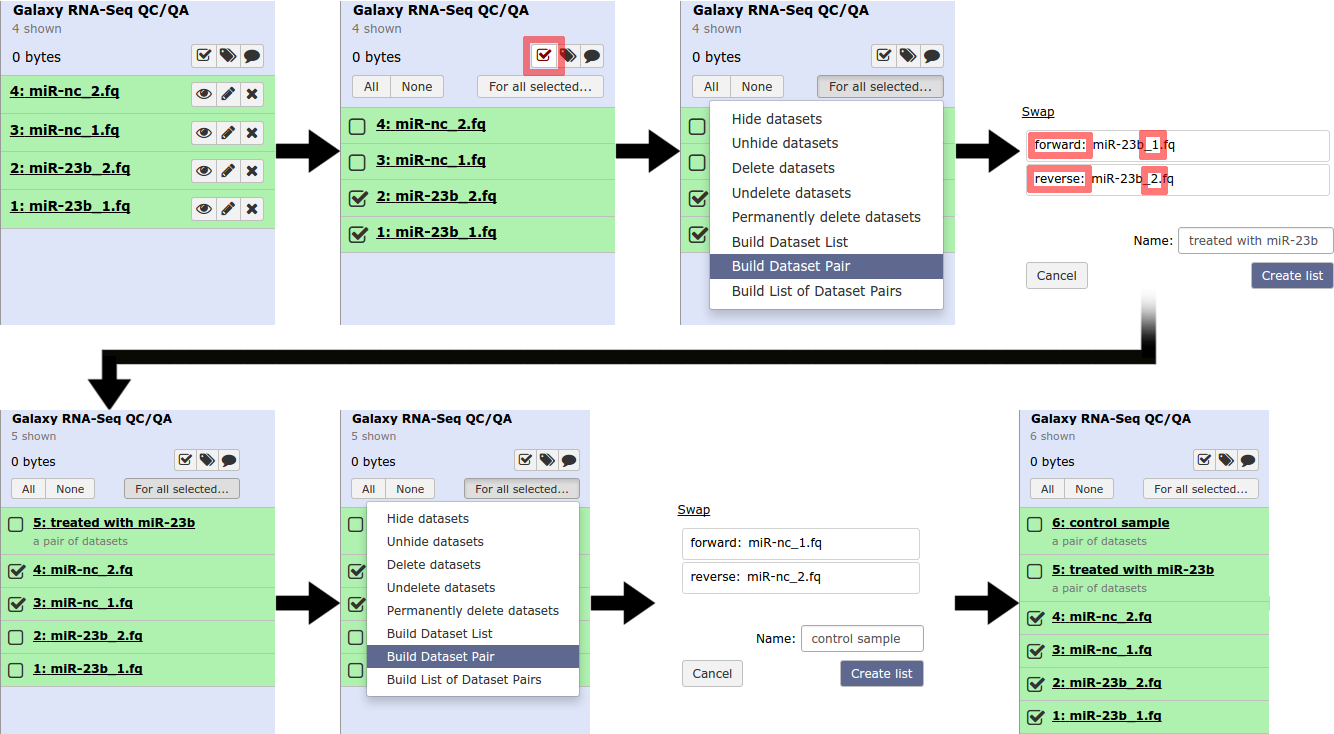
\includegraphics[width=\textwidth]{figures/qc_02.png}\\
\subsection{Fastq, Fastqsanger and FastQC}
To obtain statistics on the data, find the tool ``\textit{\underline{FastQC} Read Quality reports}''. This tool, originally developed for DNA-Seq analysis, makes several summaries of the data and reports the summary in a HTML page. By default FastQC selects the individual fastq files for analysis. This is because FastQC does analysis just on one fastq file. When we choose to select one of our pairs, galaxy will run FastQC twice and merge the results into a new pair. You can choose whether you want to run them as pair or as single file seperately, but make sure you run all of them to get an impression of the data. In the following figure it is demonstrated how to use FastQC in combination with pairs:\\
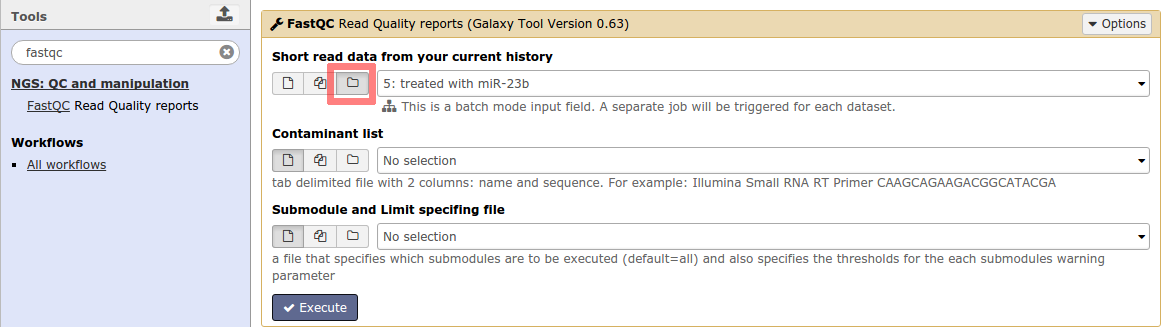
\includegraphics[width=\textwidth]{figures/qc_03.png}\\
What follows is a quality report (raw data and HTML report) for each FASTQ file. Open the miR23b (forward) FastQC report that contains \textit{\ldots: Webpage \ldots} in its name which should look similar to this:\\
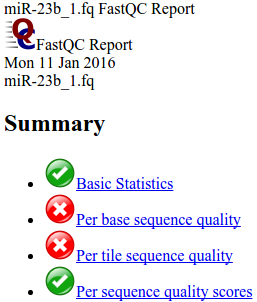
\includegraphics[scale=0.65]{figures/qc_04.png}\\
The galaxy history items are in the \textbf{fastq} format. This format is a general format that covers four specific subformats that differ in their quality encoding. Before we proceed with the next step it is important to understand the FASTQ encoding formats. They are described at the following website in section \textit{Encoding}:\\
\url{http://en.wikipedia.org/wiki/FASTQ\_format#Encoding}\\
In the FastQC report, scroll down to \textbf{Basic Statistics} and figure out what the \text{Encoding} is. This information is important because other tools want the specific subdatatype instead of `\textit{fastq}', so write the format as reported by FastQC down:\\
\verb|.......................................................|\\
The more or less standard encoding is \textit{fastqsanger}, which is the same encoding as \textit{Illumina 1.8} and \textit{Illumina 1.9}, also referred to as \textit{Illumina 1.8+}. To convert a fastq file into \textit{fastqsanger}, we use the tool ``\textit{\underline{FASTQ Groomer} converts between various FASTQ quality formats}''. In here, make sure the quality encoding you wrote down matches the one in the input field. Further, make sure you run it for each sample:\\
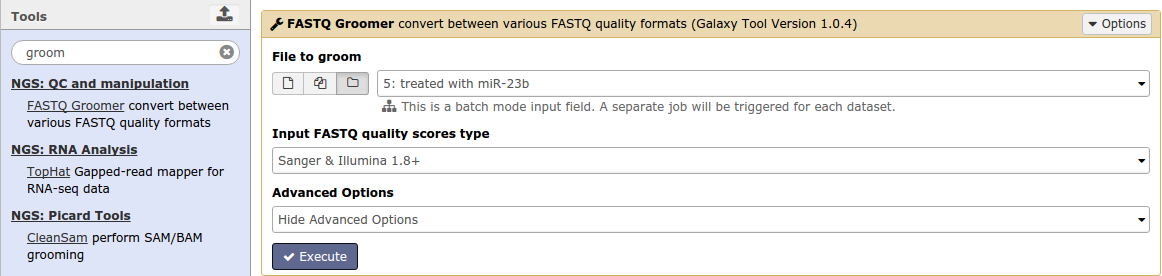
\includegraphics[width=\textwidth]{figures/qc_05.png}\\
This will add the groomed fastqsanger files to your history, with names that are not convenient. Please rename such that you can keep track of the sample name (miR23b/control) and, if you did not use pairs, whether the reads are forward or reverse.

If we go back to the FastQC webpage report, and look in section \textit{Per base sequence quality}, we see the average quality per base for all reads. The colors green, orange and red indicate whether the quality is considered good, okay, or bad. As you can see, the quality drops as the sequences get longer. It is important to realize that low quality bases will complicate alignment as well as SNP detection, because there will be more mismatches. To improve overall the base quality of the data, we would like to:
\begin{itemize}
	\item Trim the low quality bases from the ends
	\item Remove reads of which the average quality is too low
	\item Remove reads that are too short
\end{itemize}
A tool that covers all of this is ``\textit{\underline{Sickle} windowed adaptive trimming of FASTQ data}''. Because we have paired end data, we have to run it twice, once for miR-23b and once for the control. Run it with the following settings:\\
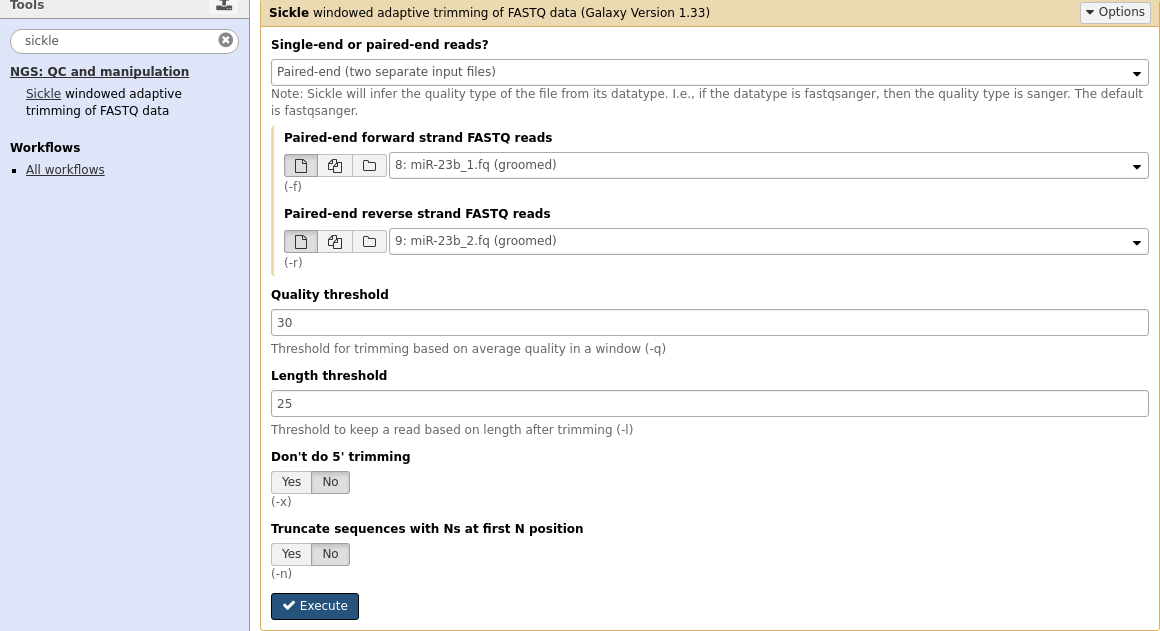
\includegraphics[width=\textwidth]{figures/qc_06.png}\\
After running a sickle analysis, rename the files 
\textit{Singletons from paired-end ...} and \textit{Paired-end output of Sickle on ...} to e.g.:
\begin{itemize}
	\item[] for miR-23b:
	\begin{itemize}
		\item miR-23b, singletons(clean)
		\item miR-23b\_1 (clean)
		\item miR-23b\_2 (clean)
	\end{itemize}
	\item[] for control sample:
	\begin{itemize}
		\item control sample, singletons(clean)
		\item control sample\_1 (clean)
		\item control sample\_2 (clean)
	\end{itemize}
\end{itemize}
If desired, you can hide the other results, such that you will get a history similar to:\\
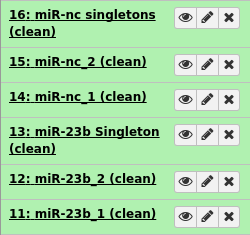
\includegraphics[scale=0.55]{figures/qc_07.png}\\
As you can see, Sickle produces for every set of paired sequencing reads, a set of pairs and an extra file with ``singletons''.
\begin{itemize}
	\item What would singletons be?
\end{itemize}
To confirm that the base quality has improved, run the FastQC again on \textit{ miR-23b (clean) }, and take a look at it:
\begin{itemize}
	\item Has the \textit{Per base sequence quality} improved?
	\item Have the per sequence quality scores improved?
	\item Why has the \textit{sequence length distribution} changed?
\end{itemize}
FastQC also has a section \textit{Overrepresented sequences}, indicated in red with a huge list. Apart from that we are using a truncated artificial dataset, it often happens in RNA-Seq data that these sequences appear. As said before, this tool was orignally written for DNA-Seq data.
\begin{itemize}
	\item Could you think of a reason why sequences could be overrepresented in RNA-Seq data?
\end{itemize}


% Module alignment:
\section{RNA-Seq: alignment}
To make more sense of the RNA-Seq data, we try to find the sequences back in the reference genome (mapping, aligning). The reference
genome should represent the most common sequence of the chromosomes of the human population. Please read the first paragraph (3 scentences) of the following url: \url{http://en.wikipedia.org/wiki/Reference_genome}
\begin{itemize}
	\item On how many individuals is hg19 based?
\end{itemize}
For RNA-Seq we need specialized RNA aligners, able to cope with gaps that originate from splicing. For this exercise we will make use of a tool called RNA-STAR. There are quite some of these aligners around. We will make use the tool ``\textit{\underline{HISAT2} A fast and sensitive alignment program}''. Load the aligner, select the following settings and leave the rest on default, and run an alignment for \textit{miR-23b (clean)} and \textit{control sample (clean)}. \textbf{Alignment is a computational very very heavy task so do NOT re-run or load it twice, or you have to give a treat:}\\
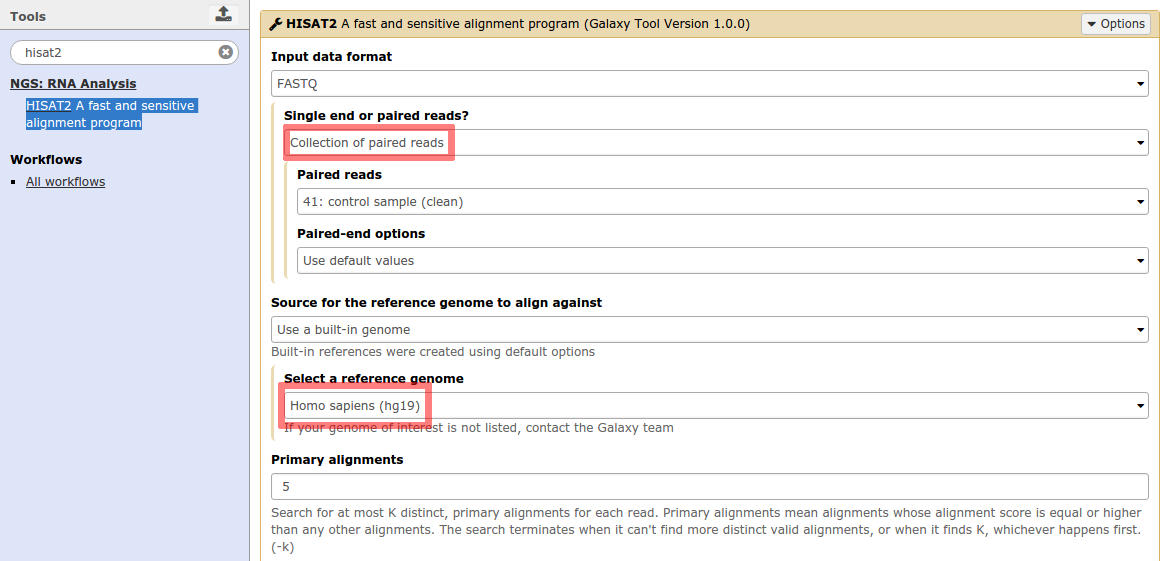
\includegraphics[width=\textwidth]{figures/alignment_01.png}\\
Please rename the \textit{HISAT2 on ...} to ``\textit{HISAT2 on miR-23b}'' and ``\textit{HISAT2 on control sample}''.
If the alignments do not have their \textbf{database} set, change it to hg19 as follows:\\
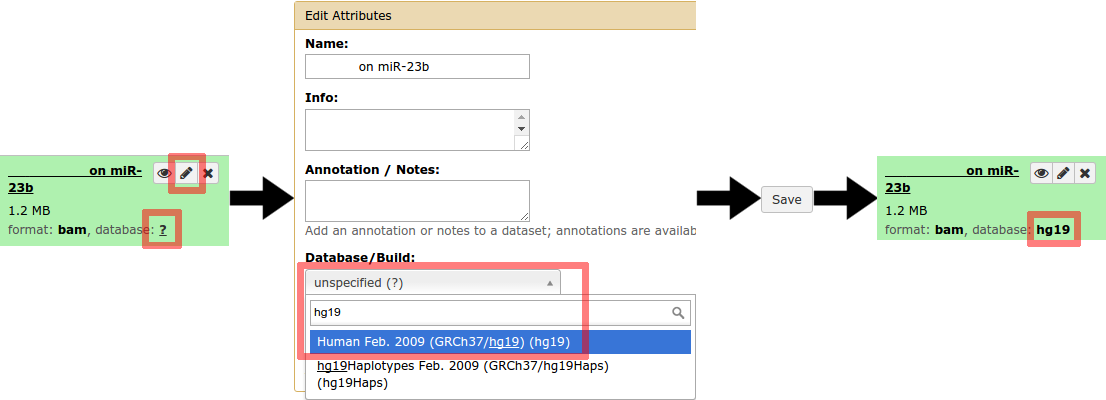
\includegraphics[width=\textwidth]{figures/alignment_02.png}\\
To get some general alignment statistics, run the tool ``\textit{\underline{Flagstat} tabulate descriptive stats for BAM datset}'' on \textit{HISAT2 on miR-23b}.
\begin{itemize}
	\item How many reads are multi-mapping?
\end{itemize}
For now we have only seen FastQ data and some summaries. To get an idea of what has been measured during the experiment, we can visualise the alignment. So, in the HISAT2 step we have been looking into hg19 where these sequences can be found in the reference genome, and this information is stored in those bam files. Import from the Shared Data library (TraIT Galaxy Training Materials $\rightarrow$ TraIT Galaxy Training - 3: RNA-Seq Tuxedo Pipeline) the file ``\textit{ucsc\_refseq.gtf}'' into your history. Start the built-in visualization Trackster at one of the alignments (make sure the dataset has \textbf{hg19} as database because we aligned to that):\\
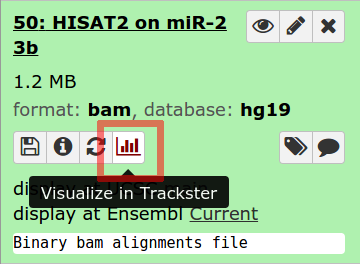
\includegraphics[scale=0.55]{figures/alignment_03}\\
Give it a name, press \textit{Create} and you will see a yellow bar, indicating that the bam file is being prepared. This means that the bam file is being convert into a file format that the browser can visualize. 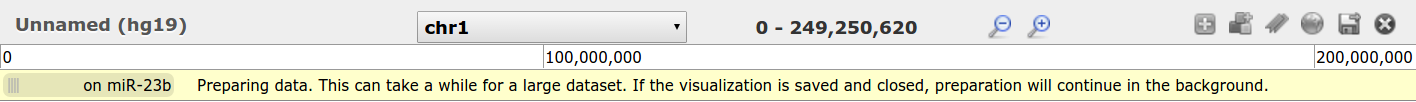
\includegraphics[width=\textwidth]{figures/alignment_04.png}\\
When this job is done, and it looks like this, make sure you save it:\\
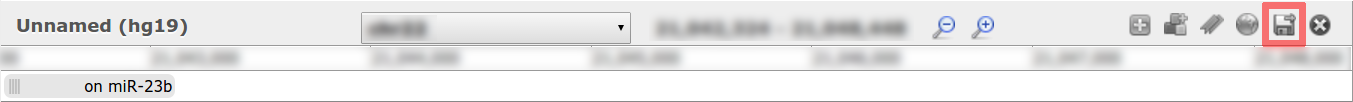
\includegraphics[width=\textwidth]{figures/alignment_05.png}\\
To add the other alignment, press the \textbf{[+]}-button:\\
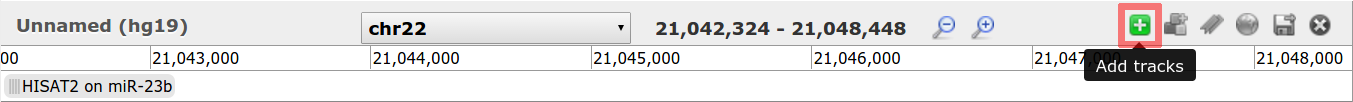
\includegraphics[width=\textwidth]{figures/alignment_06.png}\\
Now select the other alignment and press \textit{Add} and save it again:\\
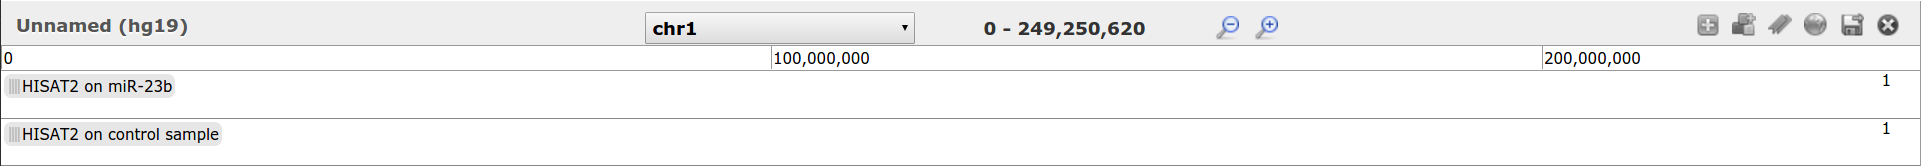
\includegraphics[width=\textwidth]{figures/alignment_07.png}\\
Remark that this is truncated data and you are supposed to see barely anything in here. Go to \textit{chr16}, to region \verb|chr16:15696870-15745667|.
\begin{itemize}
	\item Can you see where the introns and exons are located?
\end{itemize}
To help you answer this question, you can add ``\textit{ucsc\_refseq.gtf}'' that will visualize the exons and gene structure of a refseq gene annotation. It will only be visible if its database of the history item is set to hg19. Again, ensure this visualization is saved:\\
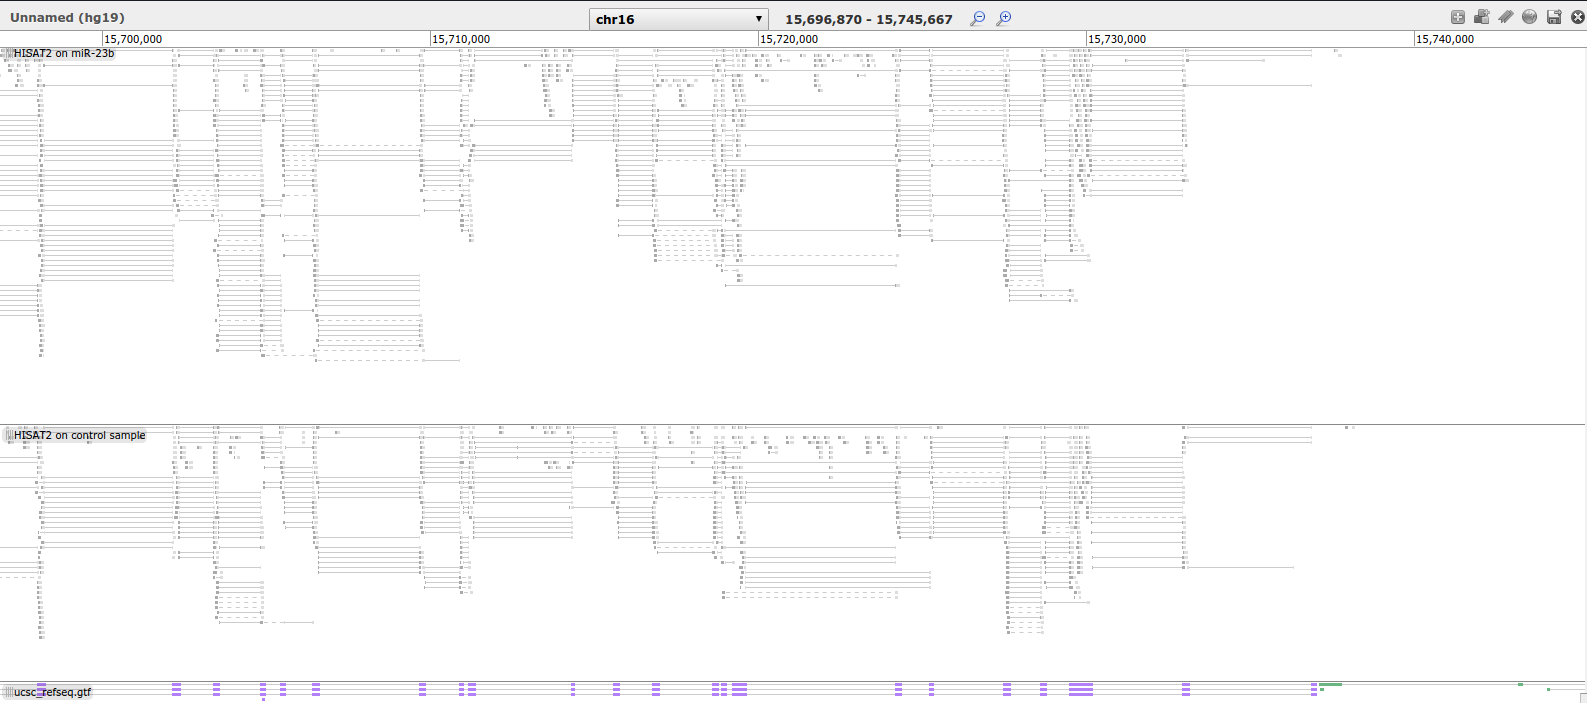
\includegraphics[width=\textwidth]{figures/alignment_08.png}\\
\begin{itemize}
	\item Can you go to \verb|chr15:60688011-60688099|, and explain what is going on there?
\end{itemize}
In the last question you can clearly see that you can observe biological facts from alignments where you couldn't extract this from the plain fastq files. Because looking through these alignments is way to much work and prone to errors, we use these bam files for a variety of computer programs to estimate metrics. These metrics can be insert size, expression levels, indel ratio's, etc., that may be used to test different hypotheses.

%The insert size is the size between the mate pairs in the alignment. Since the fragments (original part of RNA) are size selected, this should also be reflect in the alignment. Leave Trackster and run the Picard tool: ``Insertion size metrics for pairedd data''.

% @ todo
%- Ask question about insert size

\section{Expression analysis (basic)}
There are several tools able to do differential gene expression analysis, like CuffDiff, EdgeR and DESeq2, all available for Galaxy. For this analysis we will start use CuffLinks and CuffDiff and use the data created in the alignment exercise. If you were not able to make ``HISAT2 on miR-23b.bam'' and `` HISAT2 on control sample.bam'', you can import them from the data library:\\
\datalibrarydirrnaseqtuxedo \\
Simetimes it can be handy to obtain some extra details from your BAM files, for example if they are given to you by a third party. Find the tool ``BAM-to-SAM" and select the following settings:\\
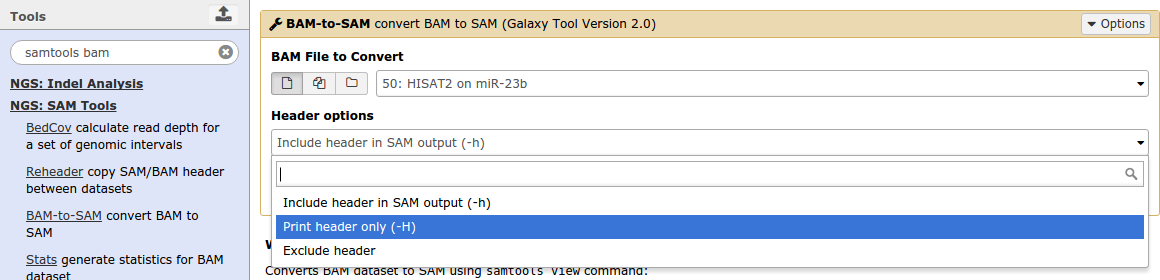
\includegraphics[width=\textwidth]{figures/basic_01.png}\\
\begin{itemize}
	\item Can you find out what version of HISAT2 was used?
\end{itemize}
As you might have seen when we visualized the alignments, it is not really feasible to find expression levels or determine genes by `eye'. To assemble the expressed genes and estimate the corresponding expression levels we will make use of the \textit{Tuxedo pipeline}. The program CuffLinks assembles genes, isoforms, measures gene expression and sets the basis for differential gene expression analysis. Run CuffLinks on both alignments separately:\\
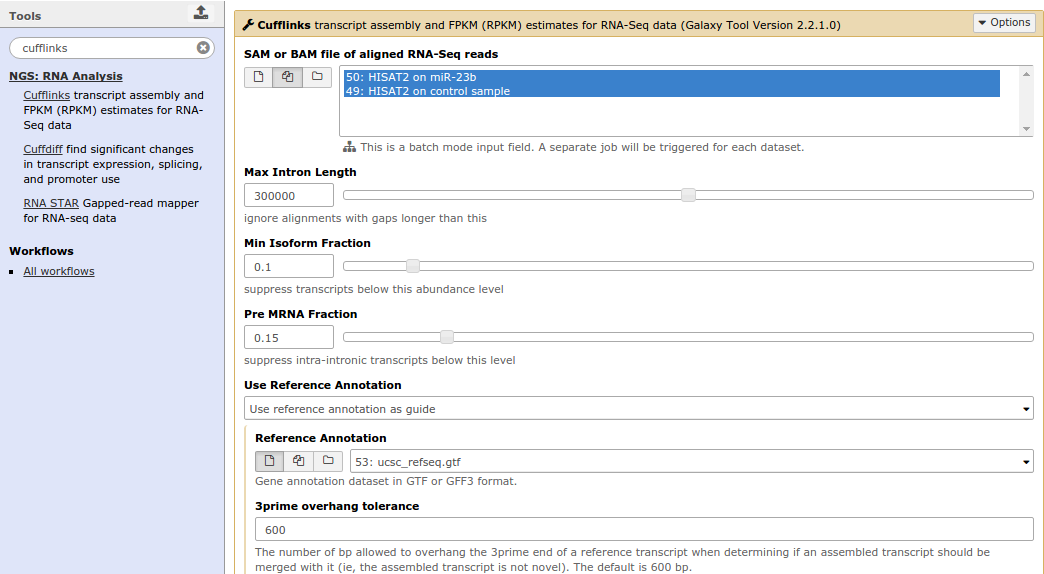
\includegraphics[width=\textwidth]{figures/basic_02a.png}\\
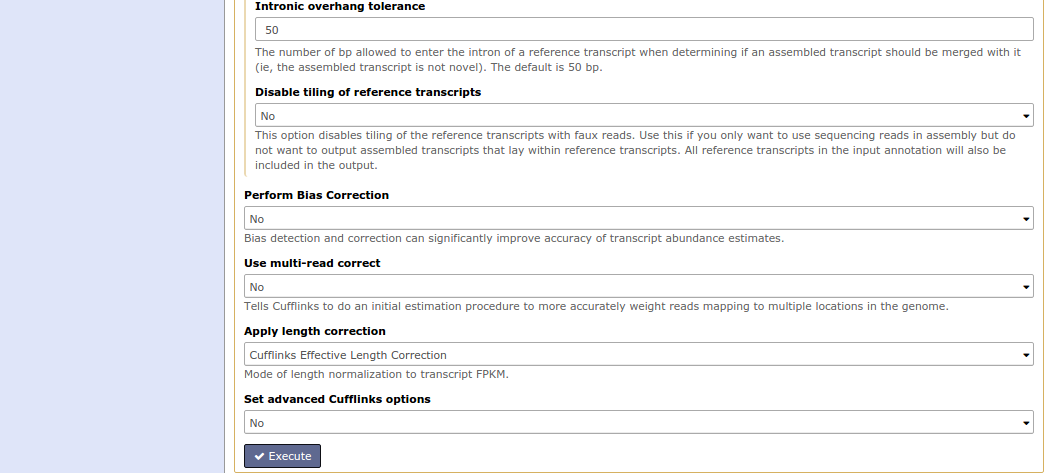
\includegraphics[width=\textwidth]{figures/basic_02b.png}\\
We have selected the \textit{Reference annotation} as guide, meaning that it uses a known gene annotation as basis for the assembled genes and adds possible new exons or genes to it. Because each sample may contain its own unique expressed transcripts, all assembled have to be merged into one transcript annotation before doing comparative expression analysis such that we can do analysis on the known (ucsc) and newly discovered transcripts:\\
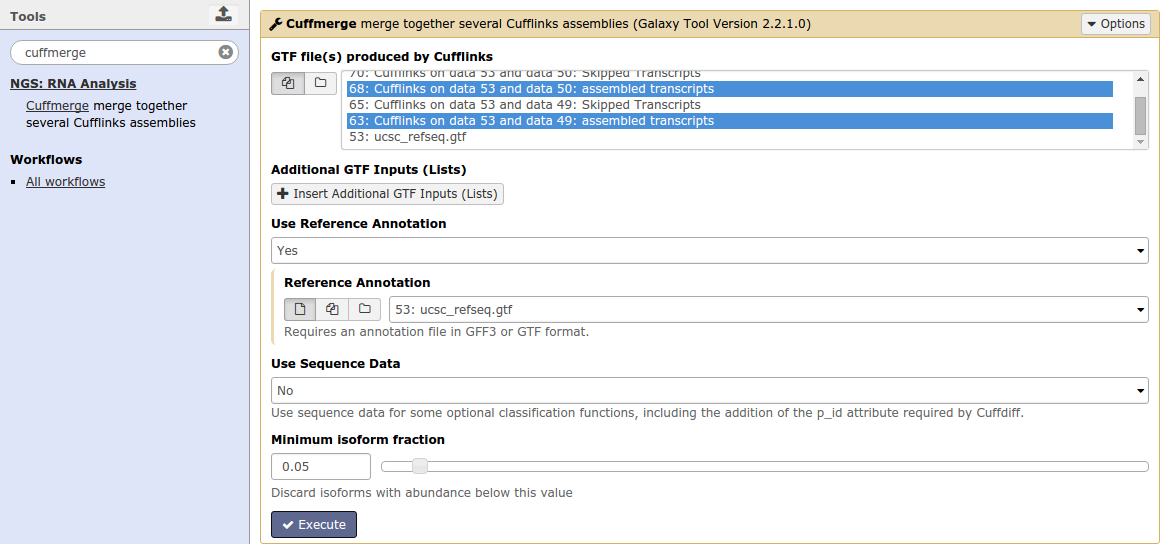
\includegraphics[width=\textwidth]{figures/basic_03.png}\\
To compare the expression profiles with each other, we use CuffDiff. Please note that we use only 1 replicate per condition which is statistically speaking a non-ideal setup. Therefore we need to set the dispersion estimation method to \textit{blind}. The next step in the pipeline will be visualizations for which CuffDiff needs to produce a database, which has to be selected by choosing \textbf{Generate SQLite} to \textit{Yes}. Proceed with the following settings and leave the rest default:\\
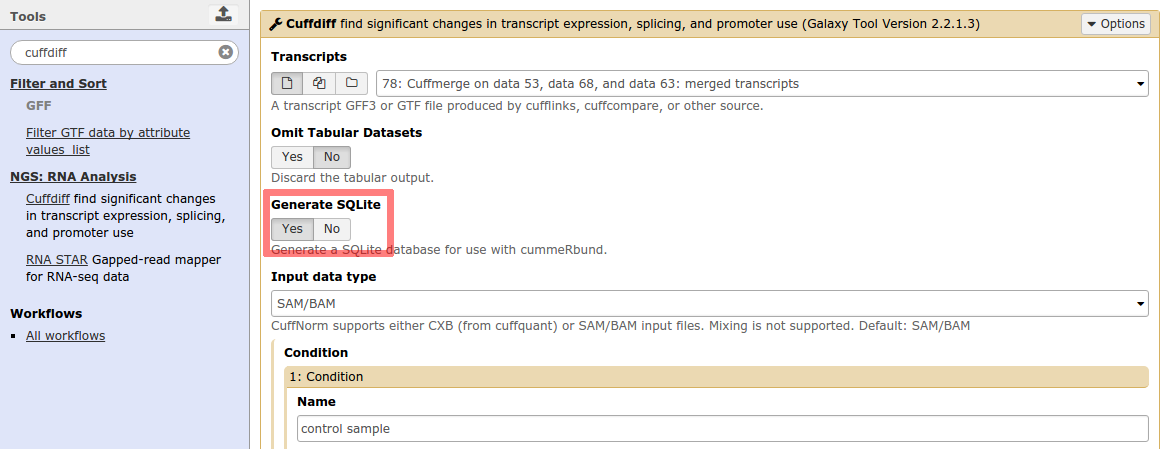
\includegraphics[width=\textwidth]{figures/basic_04a.png}\\
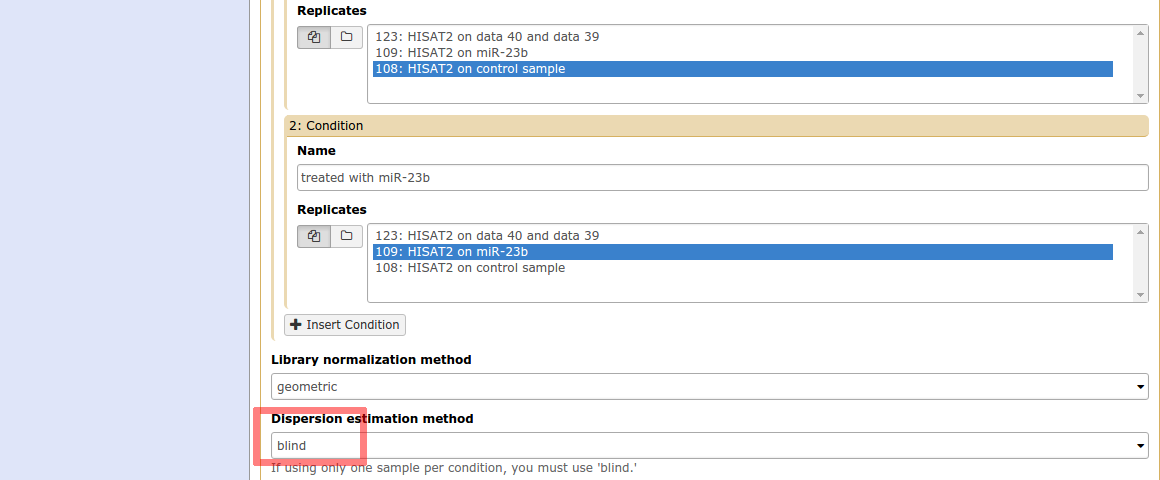
\includegraphics[width=\textwidth]{figures/basic_04b.png}\\
This analysis will create a bunch of new history items for different tests that are being applied. Look carefully before selecting the file to answer the following question:
\begin{itemize}
	\item What is the most differentially expressed gene between the sample treated with miR-23b and its control?
	\item Is there similarity with the significant genes detected in:\\\url{https://www.ncbi.nlm.nih.gov/pmc/articles/PMC3664824/figure/gkt245-F6/}
\end{itemize}
Except for CummeRbund, we have now gone through all steps of the Tuxedo pipeline individually.

\section{Expression analysis advanced}
\subsection{Estimating gene expression}
For this practical we need a RNA-seq alignments we previously made in the basic expression analysis: ``\textit{HISAT2 on miR-23b.bam}''. If you did not do that practical, you can find it in the supplementary material: \\
\datalibrarydirrnaseqadvanced $\rightarrow$ HISAT2\\
Ensure that the file is annotated at reference genome hg19. To estimate expression in RNA-Seq, we can simply count the number of reads that are aligned to each gene from the list of candidate genes. Therefore you also need to import:
\datalibrarydirrnaseqtuxedo $\rightarrow$ ucsc\_refseq.gtf\\
This list is provided as a GTF/GFF file. There are a variety of tools available for counting reads. FeatureCounts is one of the fastest and it works directly using BAM files. If you search for
``\textit{\underline{featureCounts} Measure gene expression in RNA-Seq experiments from SAM or BAM files.}'' in the Tools menu, you can find the wrapper by the name:\\
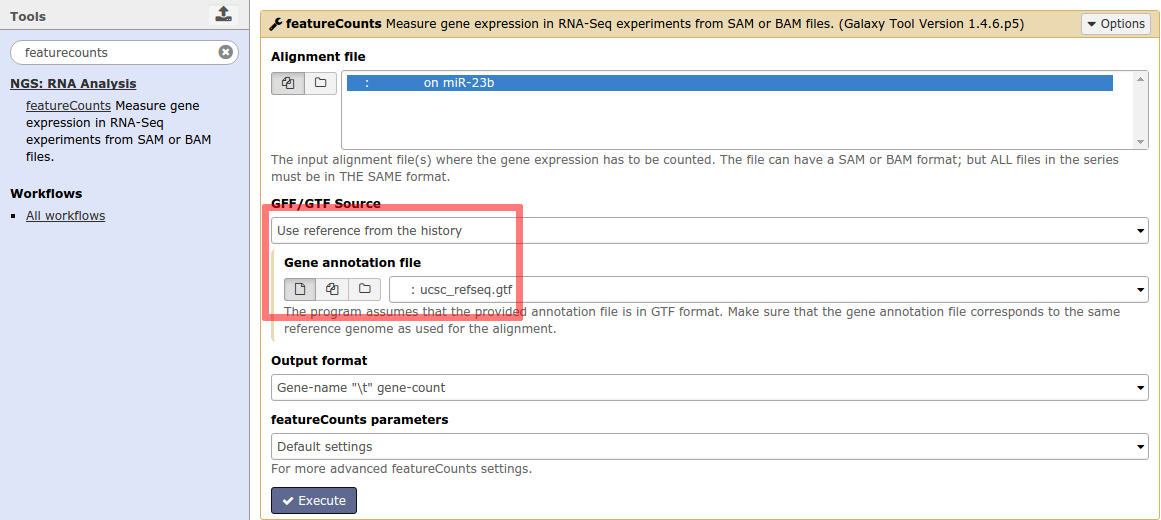
\includegraphics[width=\textwidth]{figures/expression_01.png}\\
Before we proceed, we would like to know whether the analysis has been performed correctly. Therefore we take a look at featureCounts’ output-summary file ``\textit{featureCounts on \ldots}'':
\begin{itemize}
	\item How many reads are \textit{Assigned}?
	\item How many reads are \textit{UnAssigned (sum of all)}?
\end{itemize}
The flagstat exercise told us we had 18258 reads in total. This should match with the total number of reads in the summary file as well. If we want to look at a particular gene, we truncate the large table and only show the row with the gene of interest. To filter a tabular file we proceed with the following Galaxy tool: 
\textit{\underline{Filter} data on any column using simple expressions}:\\
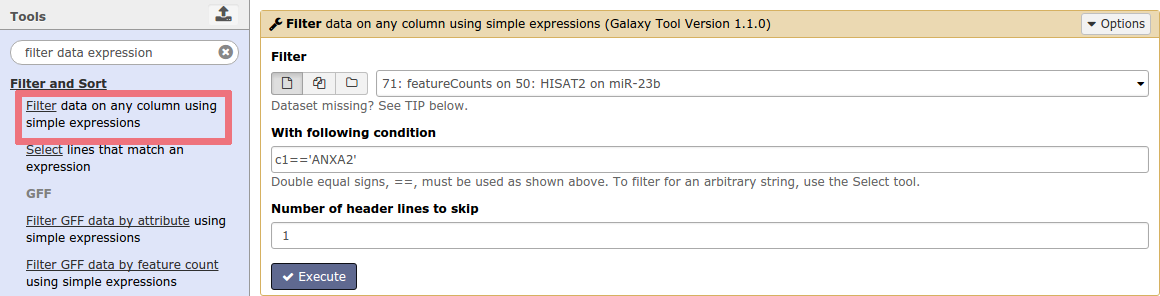
\includegraphics[width=\textwidth]{figures/expression_02.png}\\
\begin{itemize}
	\item How many reads are aligned to ANXA2?
	\item What gene has the highest gene count (tip: use \textit{sort})?
\end{itemize}

\subsection{Expression analysis: Low sequencing depth}
In the previous exercise we found which gene had the highest readcount, but what does it mean if this gene always has a high readcount in every sample? To say something about expression levels, we should say it in a context relative to other expression levels. Therefore, we need normalization and apply statistical testing. A popular package that allows to do this is EdgeR.

In the following analyses you will determine the differentially expressed genes in the MCF7-cell line between samples that have been treated with the hormone $\beta$-estradiol (E2) and those that were left as control. For this analysis we will make use of samples all taken from this cell line. In the corresponding article, the statistical power has been estimated at different sequencing depths (subsampling) and with a different number of replicates. Before we proceed, please read the abstract of the following article:
\url{http://dx.doi.org/10.1093/bioinformatics/btt688}\\
Tip: Look up where MCF7 cell lines originate from if you don't know this.\\
\\
In the article it is stated that for differential gene expression analysis it is very important to have a high number of replicates per condition. We will repeat a part of their experiment, to illustrate their findings. For this practical we have the readcounts for a sequencing depth of $\sim$30M (full), 10M and 5M, for each replicate, already made available. Each analysis in this assignment
will be to determine the number of differentially expressed (DE) genes and add this number to Table \ref{tab:dge_ad_01}:
\begin{table}[]
\centering
\caption{results of DGE analysis}
\label{tab:dge_ad_01}
\begin{tabular}{ | l | l | r | }
\hline
Replicates & Seq. Depth & Significant DE genes \\
\hline
0          & 0          & 0\quad\quad \\
7rep\_5M   & 5,000,000  & \verb|.......| ? \\
7rep\_10M  & 10,000,000 & \verb|.......| ? \\
7rep\_30M  & 30,000,000 & \verb|.......| ? \\
5rep\_30M  & 30,000,000 & \verb|.......| ? \\
\hline
\end{tabular}
\end{table}
Import the following files from data library \datalibrarydirrnaseqadvanced :
\begin{itemize}
	\item[] \verb|GSE51403_expression_matrix_5M_coverage.txt|
	\item[] \verb|GSE51403_expression_matrix_10M_coverage.txt|
	\item[] \verb|GSE51403_expression_matrix_full.txt|
	\item[] \verb|GSE51403_expression_matrix_full_5x5.txt|
	\item[] \verb|GSE51403_design_matrix_subsampled.txt|
\end{itemize}
Please take a look at the file GSE51403\_design\_matrix\_subsampled.txt.
\begin{itemize}
	\item Given that the first column lists the names of the samples and the second column the samples' corresponding condition, how many conditions does the experiment have?
\end{itemize}
\subsubsection{Subsampled datasets: 5M, 7+7}
We have a two classes problem: the class itreated with estradiol is called “ E2”, and the
other called “Control”. The design matrix provides the mapping from the RNAseq
counts per sample to the phenotype class each is associated with. Take a look at the
design matrix and see if you can find samples that belong to those classes.
\begin{itemize}
	\item [$\square$] Load ``\textit{\underline{edgeR: Differential Gene(Expression) Analysis} RNA-Seq gene expression analysis using edgeR (R package)}
	\item [$\square$] Choose \textbf{Analysis type}: \textit{Multigroup test and/or complex designs with e.g. blocking}
	\item [$\square$] Choose \textbf{Expression (read count) matrix}: {\scriptsize \verb| GSE51403_expression_matrix_5M_coverage.txt|}
	\item [$\square$] Choose \textbf{Design matrix}: \verb|GSE51403_design_matrix.txt|
	\item [$\square$] Define contrast: this is the more complicated part of the wrapper. It is defining the hypothesis we want to test. This is done via a mathematical formulation in a format described by a well known package \textit{limma}. For two class problems it is very simple: \textit{classNormal-classTreated} which in our case is: \textbf{Control-E2} (case sensitive!)
	\item [$\square$] Set \textbf{Report differentially expressed genes} to \textit{Only significant (defined by FDR cutoff)} and ensure the cutoff is set to \verb|0.01|.
	\item [$\square$] Don't select additional output files and leave the rest default.
\end{itemize}
It is always important to check whether what we did was correct. Take a look at the file ``\textit{edgeR DGE on 1: GSE51403\_design\_matrix.txt differentially expressed genes}''. If everything is correct, the gene \verb|GREB1| is located in the top of the file. Please check its corresponding gene cards page:\\
\url{http://www.genecards.org/cgi-bin/carddisp.pl?gene=GREB1}\\

\begin{itemize}
	\item Can you find on the gene cards page a regulatory factor of the gene that relates
to the E2 treatment?
	\begin{itemize}
		\item Hint: whxat was E2 again?
	\end{itemize}
	\item Can you find on the gene cards page an association with MCF-7 cells?
	\begin{itemize}
		\item Hint: what was MCF-7 for type of cell line again?
	\end{itemize}
\end{itemize}
The answers to the questions should confirm that what we find with the DGE analysis is in agreement with the setup of the analysis. In the output file, each line represents one gene indicated by the gene symbol in the 2nd column. The P-value is a probability that represents the chance to find the expression values that belong to the gene given that
they are from the same condition. The FDR is a multiple testing correction of the P-value and is usually used instead of the P-value. The lower this value, the less likely it is that the observed values are derived from the same condition. Thus, differentially expressed genes will have a low FDR and P-value. To distinguish between differences
considered to be caused by chance and differences that are that significantly large that they are considered to be from different conditions, we make use of a cut-off, commonly set to < 0.01 or <0.05.

In edgeR we have already selected to only return those genes with a FDR $\leq 0.01$. Hence, the number of lines in the history, minus 1 (header line) should give us the number of differentially expressed genes.
\begin{itemize}
	\item How many genes are significant differentially expressed between Control and E2? 
	\begin{itemize}
		\item[$\square$] Please fill this in into Table \ref{tab:dge_ad_01}.
	\end{itemize}
\end{itemize}

\subsubsection{Subsampled datasets: 10M, 7+7}
In the previous analysis, the FASTQ files contained a total of 5.000.000 reads per sample. For the next analysis we will make use of twice that amount of raw data: 10M reads per sample, 7 samples per condition.

\begin{itemize}
	\item [$\square$] Re-run the previous job with the rerun icon
	\item [$\square$] Replace \textbf{Expression (read count) matrix}: \textit{GSE51403\_expression\_matrix\_\underline{5M}\_coverage.txt} with \textit{GSE51403\_expression\_matrix\_\underline{10M}\_coverage.txt}
	\item How many genes are significant differentially expressed between Control and E2? Is this more or less than when we used 5M reads?
	\begin{itemize}
		\item[$\square$] Please fill this in into Table \ref{tab:dge_ad_01}.
	\end{itemize}
\end{itemize}
\subsubsection{Subsampled datasets: 30M, 7+7}
In the previous analyses, the FASTQ files contained a total of 5.000.000 or 10.000.000 reads per sample. The full data set contains more or less 30.000.000 raw reads per sample.
\begin{itemize}
	\item [$\square$] Re-run the previous job with the rerun icon
	\item [$\square$] Replace \textbf{Expression (read count) matrix}: \textit{GSE51403\_expression\_matrix\_\underline{5M}\_coverage.txt} with \textit{GSE51403\_expression\_matrix\_\underline{full}.txt}
	\item How many genes are significant differentially expressed between Control and E2?
	\begin{itemize}
		\item[$\square$] Please fill this in into Table \ref{tab:dge_ad_01}.
	\end{itemize}
\end{itemize}
\subsubsection{Subsampled datasets: 30M, 5+5}
We have now ran three tests with 7+7 replicates with different sequencing depths. To see what the effects are of sample replication, we should run the same analysis with a different number of replicates. To modify expression matrices within Galaxy (both concatenating and removal) we can make use of the tool ``\textit{\underline{edgeR: Concatenate Expression Matrices} Create a full expression matrix}''. We have used all our replicates in the previous analyses and so we can reduce the number of replicates to 5+5 by simply picking a subset:\\
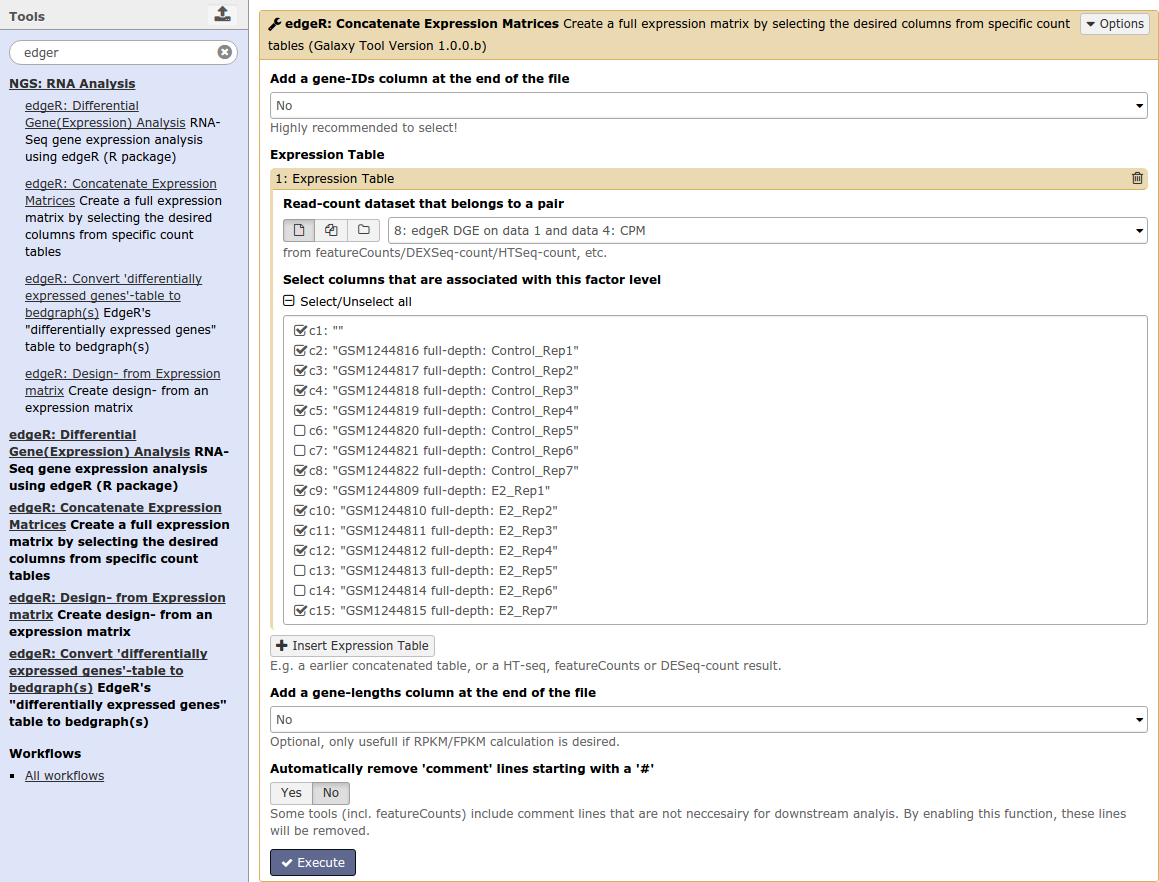
\includegraphics[width=\textwidth]{figures/expression_03.png}\\
This will create a truncated version of the expression matrix, only including the desired 5+5 replicates.
\begin{itemize}
	\item [$\square$] For convenience, rename the new expression matrix to:\\``\textit{GSE51403\_expression\_matrix\_full\_5+5\_replicates.txt}''.
	\item [$\square$] Re-run the previous edgeR DGE job with the rerun icon
	\item [$\square$] Replace \textbf{Expression (read count) matrix}: \textit{GSE51403\_expression\_matrix\_\underline{5M}\_coverage.txt} with ``\textit{GSE51403\_expression\_matrix\_full\_\underline{5+5\_replicates.txt}}''
	\item [$\square$] \textbf{Enable} the optional output: ``\textit{MDS-plot (logFC-method)}''.
	\item How many genes are significant differentially expressed between Control and E2?
	\begin{itemize}
		\item[$\square$] Please fill this in into Table \ref{tab:dge_ad_01}.
	\end{itemize}	
\end{itemize}
Take a look at the MDS plot. If you want to understand all details about MDS plots you should do some research online. For now, what matters is that the distances between the samples in the plot should correspond more or less to the distances between the samples based on the expression of all (22.000) genes.
\begin{itemize}
	\item Do you see separation between the samples from E2 and Control?
	\item Could you think of an application where it would be desired to see separation between classes?
	\item Would you expect more or less differentially expressed genes if the experiment was done on individual patient samples instead of cell-line replicates?
\end{itemize}
Can you create a tab delimited file of Table 01, e.g. in notepad or Excel, and upload it as a 'tabular' file within Galaxy? If you are not able to create the file, you can pick it from the data library. Try to open it in Galaxy as Scatterplot (visualization on the history item) and discuss with other people about the impact of removing these 2 replicates on the statistical power:\\
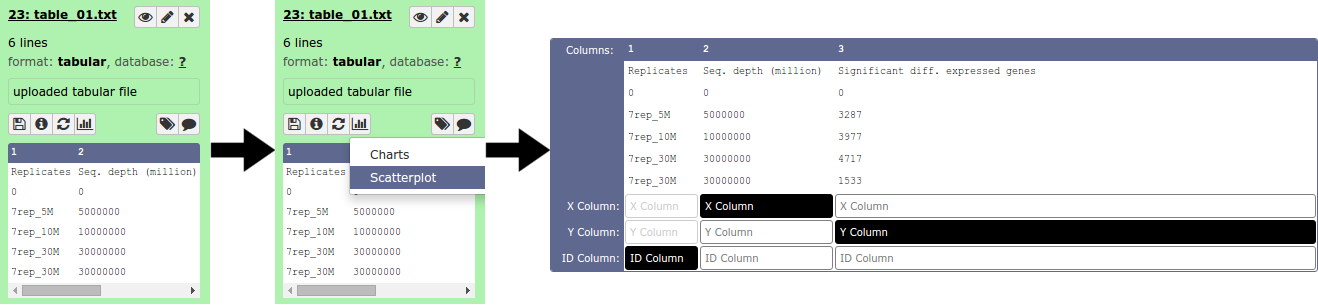
\includegraphics[width=\textwidth]{figures/expression_04.png}\\
\textbf{You are finished!}
\subsection{Bonus question}
In case you can't get enough of it, go to the Shared Data bonus section and answer the following question:
\begin{itemize}
	\item To which classes do the Unknown samples belong? (Tip: MDS / heatmap)
\end{itemize}

%\bibliographystyle{natbib}
%\bibliographystyle{plainnat}

%\newpage

\vspace{-1.5em}
\bibliography{references}

\end{document}